\documentclass[11pt, a4paper,oneside,chapterprefix=false]{scrbook}

\usepackage{a4wide}
\usepackage{times}
\usepackage{helvet}   % sets sans serif font

\usepackage{amsmath,amssymb,amsthm}

\usepackage{graphicx}
\usepackage{subfigure}  
\usepackage{fancybox} % for shadowed or double bordered boxes
\usepackage{fancyhdr}
\usepackage[dvipsnames]{xcolor}
\usepackage{rotating}

\usepackage{hyperref}
\hypersetup{
    colorlinks=true,
    linkcolor=blue,
    filecolor=magenta,      
    urlcolor=cyan,
}

\DeclareGraphicsExtensions{.pdf, .jpg, .png}
\DeclareOldFontCommand{\sf}{\normalfont\sffamily}{\mathsf}

%% macros
 \def\mathbi#1{\textbf{\em #1}}
 
% commands
\newcommand{\Adjoint}{\mbox{\rm Adj}}
\newcommand{\Area}{\mbox{\rm Area}}
\newcommand{\ACos}{{\mbox{\rm Cos}^{-1}}}
\newcommand{\ASin}{{\mbox{\rm Sin}^{-1}}}
\newcommand{\ATan}{{\mbox{\rm atan2}}}
\newcommand{\Code}[1]{{\tt #1}}
\newcommand{\Complex}{\mbox{\bf C}}
\newcommand{\Cross}{{\mbox{\rm Cross}}}
\newcommand{\Mydddot}[1]{\mbox{\shortstack{$.$\hspace*{-1pt}$.$\hspace*{-1pt}$.$\\$#1$}}}
\newcommand{\Degree}{\mbox{\rm degree}}
\newcommand{\Diag}{\mbox{\rm Diag}}
\newcommand{\Dim}{\mbox{\rm dim}}
\newcommand{\Dist}{\mbox{\rm Distance}}
\newcommand{\IntTwo}{\int\!\!\int}
\newcommand{\IntThree}{\int\!\!\int\! \!\int}
\newcommand{\Kernel}{\mbox{\rm kernel}}
\newcommand{\Kross}{\mbox{\rm Kross}}
\newcommand{\Grad}{\nabla}
\newcommand{\Perp}{\mbox{\rm Perp}}
\newcommand{\Point}[1]{{\cal #1}}
\newcommand{\Rank}{\mbox{\rm rank}}
\newcommand{\Range}{\mbox{\rm range}}
\newcommand{\Real}{{\mbox{\rm I}\hspace*{-2pt}\mbox{\rm R}}}
\newcommand{\RealSbt}{{\mbox{\rm\scriptsize I}\hspace*{-2pt}\mbox{\rm\scriptsize R}}}
\newcommand{\Res}{\mbox{\rm resultant}}
\newcommand{\Sbt}[1]{{\mbox{\rm\scriptsize #1}}}
\newcommand{\MySign}{\mbox{\rm Sign}}
\newcommand{\SignSBT}{\mbox{\rm\scriptsize Sign}}
\newcommand{\Skew}{\mbox{\rm Skew}}
\newcommand{\Span}{\mbox{\rm Span}}
\newcommand{\SqrDist}{\mbox{\rm Distance$^2$}}
\newcommand{\Trace}{\mbox{\rm Trace}}
\newcommand{\TRN}{{\mbox{\rm\scriptsize T}}}
\newcommand{\Vector}[1]{\mbox{\bf #1}}
\newcommand{\VectorM}[1]{\mbox{\boldmath $#1$}}
\newcommand{\Volume}{\mbox{\rm Volume}}

\newcommand{\IVec}{\mbox{\boldmath $\imath$}}
\newcommand{\JVec}{\mbox{\boldmath $\jmath$}}
\newcommand{\KVec}{\mbox{\boldmath $k$}}
\newcommand{\LVec}{\mbox{\boldmath $\ell$}}
\newcommand{\RMat}{{\cal R}}
\newcommand{\QMat}{{\cal Q}}
\newcommand{\QCMat}{\overline{\cal Q}}

\newcommand{\Lerp}{\mbox{\rm lerp}}
\newcommand{\Slerp}{\mbox{\rm slerp}}
\newcommand{\Quad}{\mbox{\rm quad}}
\newcommand{\Squad}{\mbox{\rm squad}}

\newcommand{\ODer}[2]{\frac{d #1}{d #2}}
\newcommand{\ODerT}[2]{\frac{d^2 #1}{d {#2}^2}}
\newcommand{\ODerM}[3]{\frac{d #1}{d #2 \, d #3}}
\newcommand{\PDer}[2]{\frac{\partial #1}{\partial #2}}
\newcommand{\PDerT}[2]{\frac{\partial^2 #1}{\partial {#2}^2}}
\newcommand{\PDerM}[3]{\frac{\partial^2 #1}{\partial #2 \, \partial #3}}

% mass density symbol
\newcommand{\Den}{\delta}

% environments
\newenvironment{BArray}[1]{\left\{ \begin{array}{#1}}{\end{array} \right\}}
\newenvironment{Combin}{\left( \begin{array}{c}}{\end{array} \right)}
\newenvironment{Matrix}[1]{\left[ \begin{array}{#1}}{\end{array} \right]}


\let\mbf=\mathbf
\let\mvec=\mathbf
\let\mcal=\mathcal
\let\mfunc=\mathrm

%\def\R{\mbox{\ensuremath{\mathrm{I\!R}}}}
\newcommand{\R}{\ensuremath{\mathbb{R}}}
\newcommand{\N}{\ensuremath{\mathbb{N}}}
\newcommand{\Z}{\ensuremath{\mathbb{Z}}}
\newcommand{\C}{\ensuremath{\mathbb{C}}}

\newcommand{\of}[1]{\left( #1 \right)}
\newcommand{\abs}[1]{\left| #1 \right|}
\newcommand{\norm}[1]{\left\Vert {#1} \right\Vert}
\newcommand{\gradient}[1]{\nabla{\!}_{#1}{\,}}
\newcommand{\twovec}[2]{\left( #1 \atop #2 \right)}
\newcommand{\threevec}[3]{\left(\begin{array}{c}#1\\#2\\#3\end{array}\right)}
\newcommand{\fourvec}[4]{\left(\begin{array}{c}#1\\#2\\#3\\#4\end{array}\right)}

\newcommand{\refsec}[1]{Section~\ref{sec:#1}}
\newcommand{\reffig}[1]{Fig.~\ref{fig:#1}}
\newcommand{\reftab}[1]{Tab.~\ref{tab:#1}}
\newcommand{\refeq}[1]{Eq.~(\ref{eq:#1})}

%\newcommand{\R}{\hspace*{0.1ex}{\sf I} \hspace{-0.3ex}{\sf R}}

%6.5
\newcommand{\eps}{\mbox{$\epsilon$}}
\newcommand{\dmin}{\mbox{$d_{\min}$}}
\newcommand{\dmax}{\mbox{$d_{\max}$}}
\newcommand{\dminmax}{\mbox{$[\dmin,\dmax]$}}

%4.2:
\def\M{\mathcal{M}}
\def\n{\mathbi{n}}
\def\p{\mathbi{p}}
\def\q{\mathbi{q}}
\def\x{\mathbi{x}}
\def\tp{^{\mathsf{T}}}

\let\vec=\mathbi%
\let\mat=\mathbf%
\let\set= \mathcal%

% Taken from (and slightly modified): http://stackoverflow.com/questions/741985/latex-source-code-listing-like-in-professional-books

\usepackage{listings}
\usepackage{courier}
\usepackage{color}
\definecolor{lightgray}{gray}{0.9}
\definecolor{commentgreen}{rgb}{0.2,0.56,0.2}
 \lstset{
         basicstyle=\footnotesize\ttfamily, % Standardschrift
         numbers=left,               % Ort der Zeilennummern
         numberstyle=\tiny,          % Stil der Zeilennummern
         %stepnumber=2,               % Abstand zwischen den Zeilennummern
         numbersep=5pt,              % Abstand der Nummern zum Text
         tabsize=2,                  % Groesse von Tabs
         extendedchars=true,         %
         breaklines=true,            % Zeilen werden Umgebrochen
         keywordstyle=\color{red},
                frame=b,         
          keywordstyle=[1]\textbf,    % Stil der Keywords
         keywordstyle=[2]\textbf,    %
         keywordstyle=[3]\textbf,    %
         keywordstyle=[4]\textbf,   %\sqrt{\sqrt{}} %
         stringstyle=\color{blue}\ttfamily, % Farbe der String
         showspaces=false,           % Leerzeichen anzeigen ?
         showtabs=false,             % Tabs anzeigen ?
         xleftmargin=17pt,
         framexleftmargin=17pt,
         framexrightmargin=5pt,
         framexbottommargin=4pt,
         backgroundcolor=\color{lightgray},
         showstringspaces=false,      % Leerzeichen in Strings anzeigen ?
         commentstyle=\color{commentgreen}
 }
 \lstloadlanguages{% Check Dokumentation for further languages ...
         %[Visual]Basic
         %Pascal
         %C
		PHP, 
         C++
         %XML
         %HTML
         %Java
 }
    %\DeclareCaptionFont{blue}{\color{blue}} 

  %\captionsetup[lstlisting]{singlelinecheck=false, labelfont={blue}, textfont={blue}}
  \usepackage{caption}
\DeclareCaptionFont{white}{\color{white}}
\DeclareCaptionFormat{listing}{\colorbox[cmyk]{0.43, 0.35, 0.35,0.01}{\parbox{\textwidth}{\hspace{15pt}#1#2#3}}}
\captionsetup[lstlisting]{format=listing,labelfont=white,textfont=white, singlelinecheck=false, margin=0pt, font={bf,footnotesize}}

\usepackage{color}
\definecolor{RED}{rgb}{1,0,0}
\definecolor{GREEN}{rgb}{0,0.7,0}
\definecolor{BLUE}{rgb}{0,0,1}
\newcommand{\FIXME}[1]{{\color{RED}{\textbf{FIX}: #1}}}

\addtolength{\textheight}{2.0cm}
\addtolength{\voffset}{-1cm}
\addtolength{\textwidth}{1.8cm}
\addtolength{\hoffset}{-.9cm}

\widowpenalty=10000
\clubpenalty=10000

\newcommand{\todo}[1]{}
\renewcommand{\todo}[1]{{\color{red} TODO: {#1}}}


\lstdefinelanguage{JavaScript2}{
  keywords={typeof, new, true, false, catch, function, return, null, catch, switch, var, if, in, while, do, else, case, break, for, forEach},
  keywordstyle=\color{orange}\bfseries,
  ndkeywords={class, export, boolean, throw, implements, import, this},
  ndkeywordstyle=\color{darkgray}\bfseries,
  identifierstyle=\color{black},
  sensitive=false,
  comment=[l]{//},
  morecomment=[s]{/*}{*/},
  commentstyle=\color{purple}\ttfamily,
  stringstyle=\color{ForestGreen}\ttfamily,
  morestring=[b]',
  morestring=[b]"
}

\begin{document}

\frontmatter
%\maketitle %automatic version
% --- selfmade version ----
\begin{titlepage}
	\setlength{\parindent}{0cm}
	\addtolength{\textheight}{1.0cm}

	\vspace{0.5cm}
	\Huge
	{\textbf{A visualization of biodiversity through time\\ }}

	\vfill \vfill \vfill
	\begin{center}
	\includegraphics*[width=0.8\textwidth]{figures/cover/cover}
    \end{center}
	\vfill
	\sf \Large
	Master Thesis \\
	\today \\[0.5cm]
	\large
	by Wuxing Dong, 18-946-038

	\vfill \vfill \vfill
	\begin{minipage}[b]{0.5\textwidth}
	Supervisors: \\
	Prof. Dr. Renato Pajarola \\
	Gaudenz Halter \\
	\end{minipage}
	%
	\begin{minipage}[b]{0.5\textwidth} \raggedleft
	Visualization and MultiMedia Lab \\
	Department of Informatics \\
	University of Z{\"u}rich
	\end{minipage}

	\vfill
	\hrule
	\vspace{0.5cm}
	\includegraphics*[width=0.3\textwidth]{figures/cover/uzh_logo} \hfill
	\includegraphics*[width=0.3\textwidth]{figures/cover/vmml_logo}
\end{titlepage}
%%

%=====================================================================

%=====================================================================
\chapter{Abstract} \label{chp:abstract}
%=====================================================================

The increasing size and dimensionality of datasets in the humanities pose new challenges to scholars working with them, including how to establish an overview over the dataset, how to establish new hypotheses and how to test them. Material, pattern, and texture usage in moving image is an attractive example of such multi-dimensional datasets in film studies, as an almost infinite number of combinations thereof are possible.\\ 
This thesis proposes interactive data visualization and exploration of film features as a solution to assist film researchers in the investigation of relationships between material, pattern, textures, and a wide range of qualitative analysis labels in a large film database. Using an array of visual components in combination with exhaustive computational methods and an interactive user-interface, the proposed solutions show to be effective in conveying the global and local structure of the dataset as well as the relationship between different feature groups of features. Finally, the resulting visualization tool is embedded into the well-established research framework of the FilmColors project.


%=====================================================================

\tableofcontents

\mainmatter


%=====================================================================
\chapter{Introduction} \label{chp:introduction}
%=====================================================================

\section{Effective visualization of data} \label{sec:one}
In the time of the information age, the Internet has become a primary source to educate ourselves about the world. It is therefore a great opportunity for the scientific community to take advantage of the web and create high quality products to communicate their findings and ideas to the non-experts and general public. Textbook-styled verbal explanations can be rigorous, however, they easily become tedious and are already made available by school and college education. Videos are based on visual learning, quick to absorb, yet there is no engagement with the viewers. An interactive data visualization can provide an excellent way for users to understand scientific concepts. New knowledge is conveyed by direct visual impact that easily draw attention, and insights can be formed by actively exploring the data and observing the response of the presentation due to the users' own actions. This learn-by-doing strategy can consolidate the new knowledge. \\

Although graphics plays a major role to deliver scientific messages, there is a lack of formal theory on producing good graphics, and domain experts tend to rely on practical experiences that are guided by certain design principles. Increasing amount of studies have focused on concluding such principles. Chen and colleagues have summarized that three main aspects to pay attention to in a visualization project are its contents, the relevance in the context of the larger whole as well as the forms and aesthetics (construction). Similarly, McCandless argued that a good visualization requires integrity of information, interestingness of story (concept), usefulness of goal and beauty of the visual form.\\

Before embarking on the production of a visualization, one should note the characteristics of human visual perception to improve the design strategies in practice. Cognitive psychological studies aimed at examining human visual attention by exposing users to certain visual processing tasks. The results of those studies suggested some guidelines for more effective visualization. When the visual features of a certain type of data is expected or previously known, the accuracy and speed of visual perception is drastically improved. Therefore, a visual feature should be assigned to the same data dimension, or type of data. It is also important to note that attention is limited and selective, therefore the amount and diversity of information should be kept within the limits of cognitive load. When many categories of data are present, compromises are needed to retain graphics complexity and only demonstrate a few number of categories at a time. \\

Through early years of research on how images are analyzed visually, it has been found that detailed vision is only achievable by actively focusing on small portion of the visual field. However, a few visual features, such as colors and curvatures, are subjected to preattentive processing, which can be effortlessly and rapidly detected by low-level visual processes. Colors is thus a powerful method in graphics. It can encode extra layers of information, and serves a leading factor to make a visualization memorable. Three major schemes for using colors are sequential, diverging and qualitative. A sequential scheme relates increasing value of the data to the intensity of the color, while using only one or two hues. In diverging scheme, two extremes are shown by two sequential schemes, and the middle or neutral value corresponds to a white or neutral color. The qualitative scheme uses a variety of distinguishable colors to represent data belonging to distinct categories. It is a good practice to choose color schemes that are distinguishable enough, such that minimal information is lost when converted into a gray scale. In addition, when a range of colors are used together, reducing the opacity of certain or all colors avoids overwhelming visual impact to the viewers. \\

Design principles have also been examined and summarized by different studies. The design process should be guided by the core messages to deliver. It is important to first prioritize what information to show, envision the final result, and then choose appropriate geometries that fulfill the objectives. Geometries are the forms in which data is illustrated, and the majority of them can be categorized into amounts, compositions, distributions or relationships. Often, different geometries can be considered on the same data, however, the most efficient geometry should be of high data-ink ratio, which is the ratio between the amount of ink allocated on the actual data to the total amount of ink used in a figure. While a high data-ink ratio indicates high efficiency, it is also important for a visualization to be simple, self-explanatory  and straight to the points, such that the viewers are not overwhelmed with too much information. \\


\section{Background on biodiversity and tectonic change} \label{sec: two}
The data this thesis chooses to visualize is biodiversity through earth history. Considering various pressing environmental issues nowadays, it is important to raise the awareness of the general public on how different forms of life came to exist and change during the course of earth history. Climate change has become a non-negligible factor influencing on our daily life and the future of human society. Recently, the world sees increasing amount of extreme weather conditions, causing significant losses in human lives and properties. The ecosystem is also under threat of a mass extinction event, after which 90\% of all species are expected to disappear, and its leading cause is considered to be human activity. 
By understanding the history of life through simple and interesting visualizations, viewers could appreciate the inseparable relationship with our environment, and be more promoted to act in a more environmentally-friendly and sustainable manner.

\subsection{Biodiversity as a result of evolution} \label{subsec: one}
\begin{figure}[h]
	\centering
	\subfigure[John Gould's sketches of the various beak shapes of the Galapagos finches as a result of evolution. ]{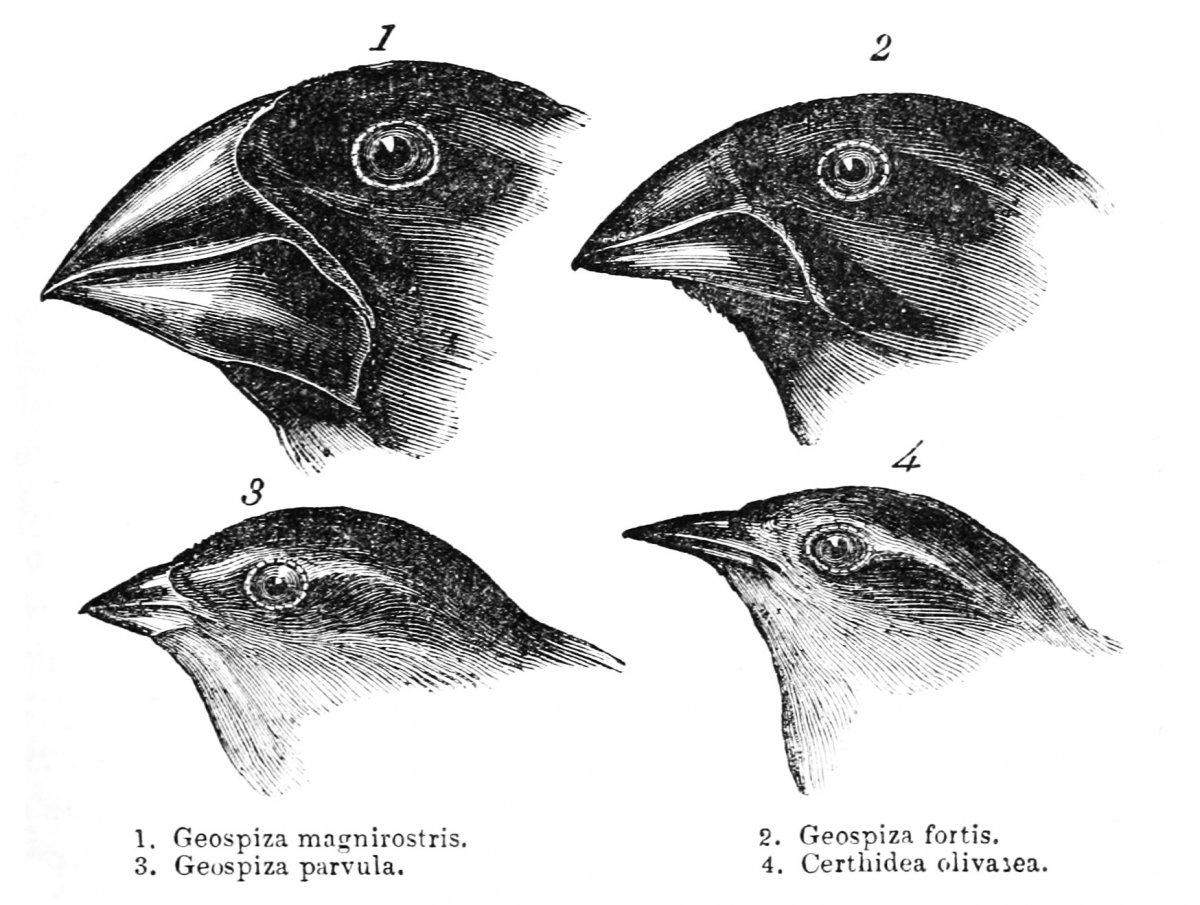
\includegraphics[width=0.45\textwidth]{figures/introduction/finches}\label{fig:finches}} 
	\hfill
	\subfigure[Biodiversity during Phanerozoic experiences non linear change with mass extinction events. ]{\includegraphics[width=0.45\textwidth]{figures/introduction/phanerozoic_biodiversity}\label{fig:phanerozoic_biodiversity}} 
	\label{fig:evolution}
\end{figure}
Current views on the process of species formation is based on modern evolution theory originated from Darwin's work. To summarize briefly, all forms of life are argued to share a common ancestor, which diversified over the course of evolution to form the current tree of life. An organism's genomic information is encoded in DNA or RNA, which is replicated over generations. However, recombination and random mutation events occur during the replication process, resulting in genetic variations, which in turn causes difference in phenotype, the observable traits of organisms. Individuals with traits that are more suitable to their particular environment are more likely to survive and pass their genes to their offspring, comparing to those that are poorly adapted to the environment. This process is termed natural selection. A classic example of evolution is the adaptive radiation of finches on the Galapagos islands. The beak shapes of the finches on different islands diversified to specialize on obtaining the dominant type of food on different islands. Over generations, species evolve as a consequence of the change in the prevalence of advantageous genes. Finally, a new species is formed during the process of speciation. It occurs when enough genetic variations are accumulated between the original population and the descendant population, such that organisms from the two groups are not capable of producing fertile offspring, namely, the two groups have reproductive isolation. \\

It is believed that life emerged from 3.5 billion years ago. The past 540 million years ago (the Phanerozoic Eon) sees rapid development and diversification of life. Throughout evolutionary history, there are records of drastic changes in biodiversity occurring in a relatively short period of time. Radiations are rapid increase in biodiversity. An example is the Cambrian explosion, during which most phylums of multi-cellular organisms appeared. On the contrary, biodiversity experiences rapid decline during mass extinction periods. There is evidence of five mass extinction periods, one of which occurred in Cretaceous and Tertiary, when the dinasours were exterminated and mammals thrived due to their selective advantage given by their fur in the cooling environments. These periods of radiation or extinction are caused by special events, plate motions, as well as change in climate, such as temperature and oxygen level. \\

\subsection{Tectonic shift as a driver of biodiversity change} \label{subsec: two}
The earth crust is composed of a number of tectonic plates undergoing constant changes. The hear generated from the interior of the planet causes the movement of the plates, as a result, earth appears very differently throughout millions of years of history. The plate motion results in new landscapes and new continents, affecting the inhabitants of lives. For instance, the current continents are thought to belong to one super continent called Pangaea, and gradually drifted away from each other since 175 million years ago. \\

As the continents separated, populations from the same species are geographically isolated into their particular environments that is created from the plate motion. Since organisms are under constant selective pressure from the environment, new species are formed in the newly created environments. An example is the distribution of ratite as a result of tectonic movement. 

\section{Source of data} \label{sec:three}
\emph{The fossil}\\
The biodiversity of ancient time periods is represented by fossil records. For this purpose, we use paleodb, which contains 1.3 million occurrences of fossil records. Each record has its unique ID, identified taxonomy, estimated maximal and minimal time (in million years) to today, and their coordinates. \\

\noindent \emph{The tree}\\
All identified species are classified in taxonomy, following the hierarchy of domain, kingdom, phylum, class, order, family, genus and species. Therefore, it can be naturally organized into a tree structure. Conveniently, for each fossil record in PBDB dataset, the names on each rank of the taxonomy is available. The highest taxonomy rank in the PBDB dataset is kingdom, namely the kingdom of Animalia (animal) and Plantae (plants). Since the two kingdoms are under the domain of Eukaryota, a rooted tree of life can be generated from the taxonomy information of all fossil record.\\

\noindent \emph{The map}\\
The geological information is provided by Matthew and colleagues, who traced the coastlines of the continents from 410 million years ago until the current world. 

\section{Aim of the thesis}
This thesis aims at building a web application that visualizes the change in biodiversity through the course of earth history. In the final product, users can view a customizable tree of life during a selected time period under a selected taxonomy. In the meantime, the fossil records belonging to the given tree of life is shown on the map, whose coastlines correspond to that of the selected epoch in ancient time. 

\section{Thesis structure}
Chapter one introduces the topic of data visualization and domain specific background information, and it claims the goal of the thesis. Chapter two analyzes some related work, indicating what could be learned and improved for the visualization to be built. Chapter three outlines the problems to be solved at each stage for building the web application. Chapter four discuses the technical solutions for data processing and web development stage, respectively. In chapter five, the implementation methods for data processing, backend and frontend are listed. Chapter six reports the result of the product. Chapter seven concludes the project and suggests future work.


%=====================================================================
\chapter{Related work} \label{chp:related_work}
%=====================================================================

There already exists an abundance of visualizations on the Internet regarding to tree of life as well as plate motion. This section selects several related work and discusses their inspirations for designing our own visualization on this topic. 

\section{Tree-based visualizations on biodiversity}
OneZoom (\url{https://www.onezoom.org/}, Fig.\ref{fig:OneZoom}) visualizes all known living things in a fractal tree, and it is targeted for both professionals and the masses. Users can zoom into or out of different levels of the tree by scrolling, and can search for a particular location in the tree by its name. 

\begin{figure}[h]
	\centering
	\subfigure[The overview of OneZoom's tree from root. ]{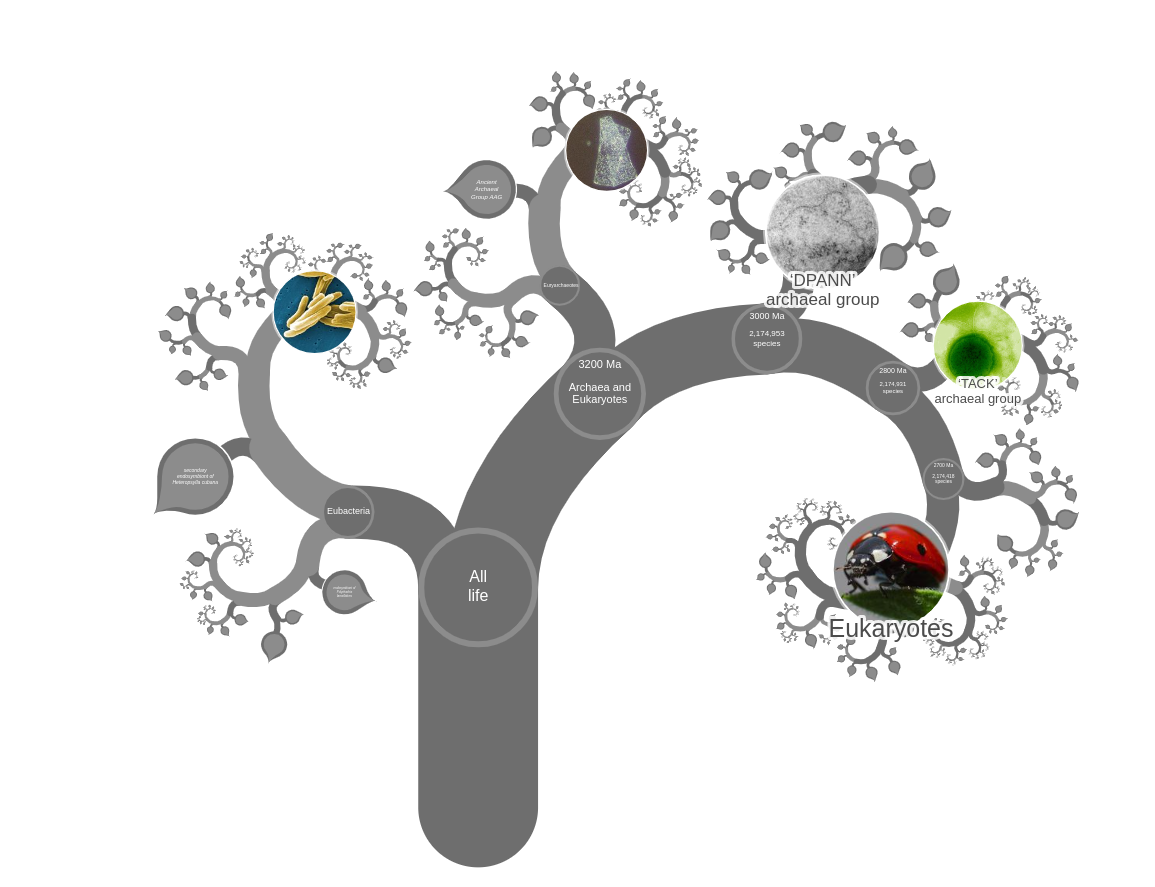
\includegraphics[width=0.45\textwidth]{figures/related_work/onezoom_overview}\label{fig:OneZoom_a}} 
	\hfill
	\subfigure[The view on OneZoom's tree when zoomed onto mammals. ]{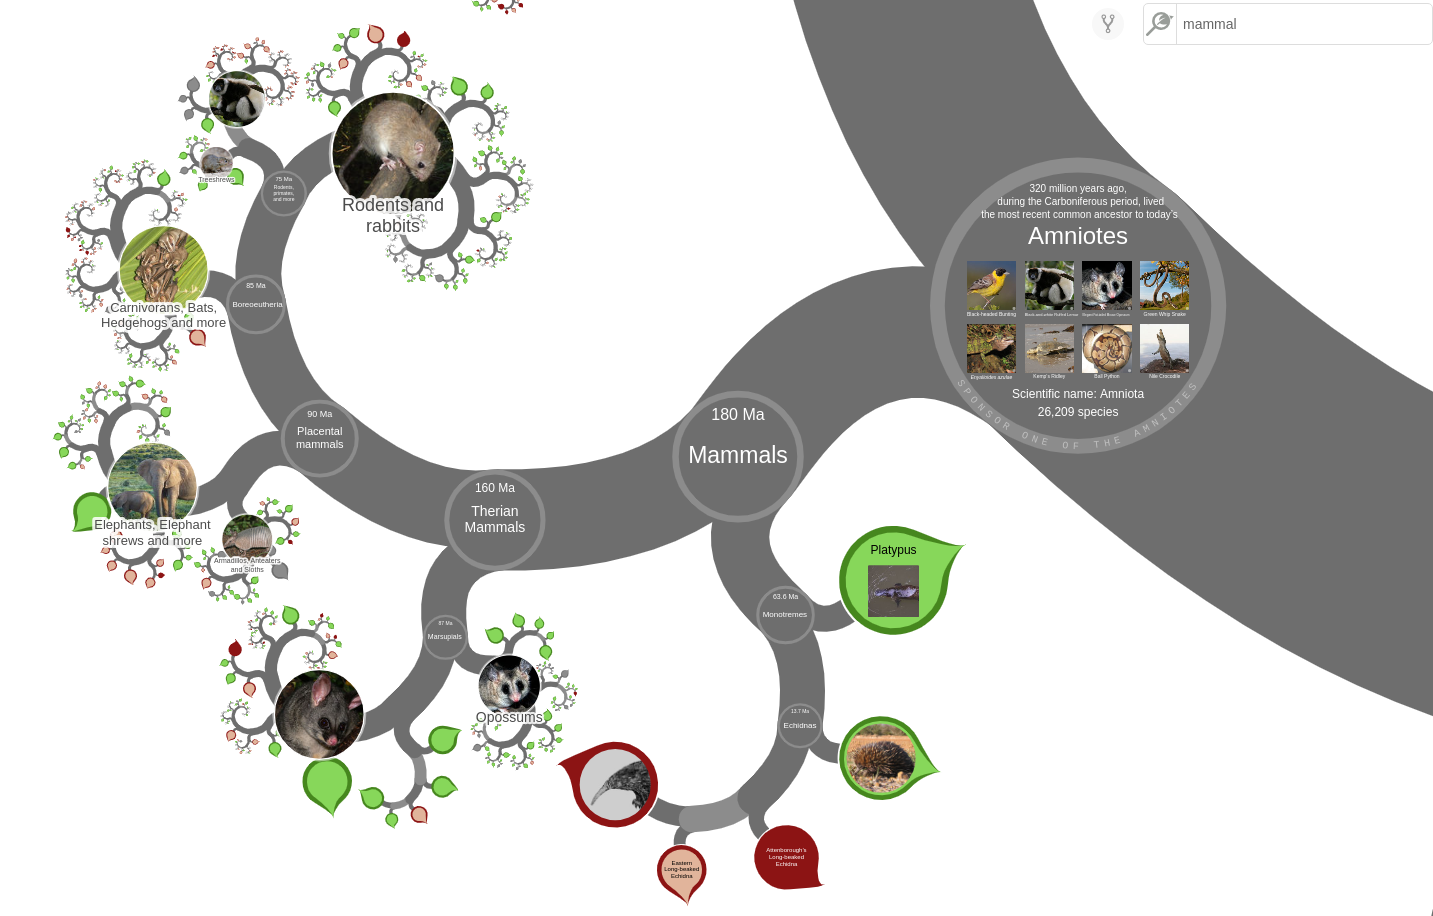
\includegraphics[width=0.45\textwidth]{figures/related_work/onezoom_mammal}\label{fig:OneZoom_b}} 
	\caption{Tree of life implementation in OneZoom. }
	\label{fig:OneZoom}
\end{figure}

The fractal design gives the tree a nice appearance, with leaves and nodes resembling the leaves and branches of an actual tree. General information such as pictures or earliest time of a node is also well packed in the interactive image. There is a reset button to return to the root, and a drop down list that provides links to the nodes along the path to root from the current position. These functions are convenient for navigation and similar functionality should be implemented in this thesis. It is claimed that all categorized organisms, which has a total amount of over two million, are included in the tree. Each species in the tree structure are incorporated with a phylogenetic classification, indicating that for a particular species represented by a leaf to reach the root, it visits all of the nodes representing each of its ancestor throughout the evolutionary history. Although how a certain organism evolved from the common ancestor of all life can be rigorously inspected, from the user experience's point of view, the tree is extremely deep. Apart from manually searching for a name, navigating to a desired location in this deep tree is mainly achieved by scrolling and dragging the item of interest to the center of the screen. This makes it difficult for viewers to relocate to a different section of the tree, or to gain an overview of where the current node or leaf sits in the entire tree of life. To reach the root (\ref{fig:OneZoom_a}) from mammal (\ref{fig:OneZoom_b}) while viewing its path, users need to scroll through all upper levels of the similar-looking spiral structures of the tree, which appears to be confusing. A similar tree of life is Lifemap (\url{http://lifemap.univ-lyon1.fr/explore.html}), which ameliorates the navigation difficulty by highlighting the ancestry path from root to an entry (Fig\ref{fig:lifemap}). However, due to the sheer depth of the tree, users still need to travel deep into the tree by scrolling. Rather than demonstrating the exact ancestral paths, the purpose of the tree for this project is to organize each species such that biodiversity can be viewed in an intuitive way. As a consequence, all entries can be organized in only the main taxonomic ranks, limiting the tree's depth to be eight and thus simplifying the navigation process. In addition, to avoid scrolling and dragging, the tree can take a fixed position, while where a node or leaf locates can be shown in a clickable breadcrumb structure that provides an overview of the whole tree. \\

\begin{figure}[h]
	\centering
	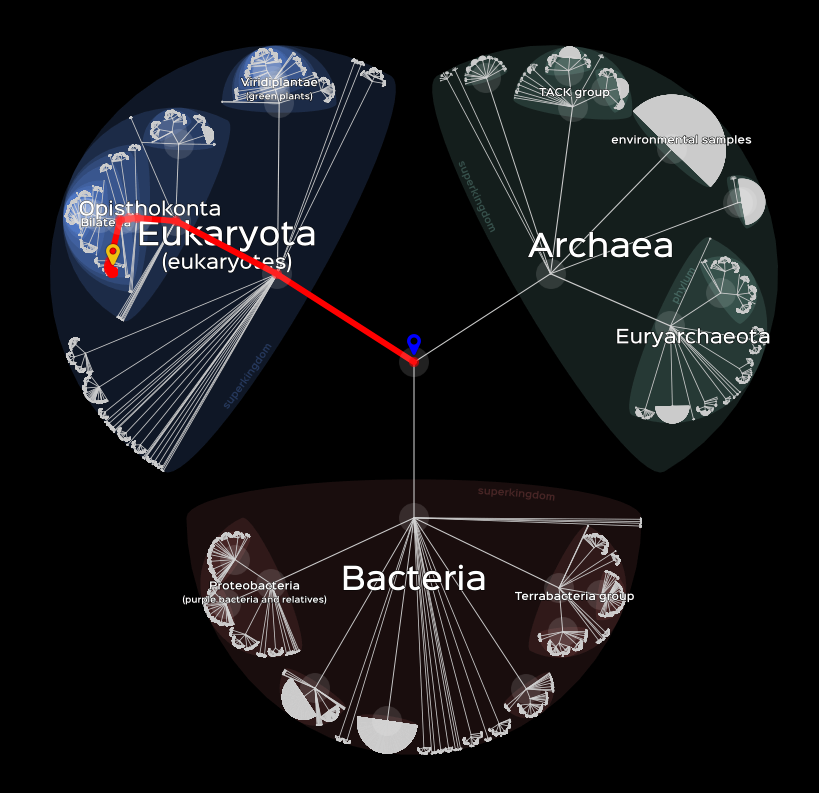
\includegraphics[width=0.5\textwidth]{figures/related_work/lifemap}
	\caption{Lifemap enables a "path from root" functionality that highlights the ancestry path from \textit{Homo sapiens} to the root. }
	\label{fig:lifemap}
\end{figure}

A much simplified version of tree of life is Evogeneao (\url{https://www.evogeneao.com/en/explore/tree-of-life-explorer}), which is intended for school education. As shown in Fig\ref{fig:evogeneao}, all species are grouped into clearly colored groups, which gives the viewers a direct and memorable visual impact. A similar design could be adapted in this project. With the tree of life arranged in a half circle that is labeled with time and a few iconic events, users could get a view of how life radiated from the common ancestor into great diversity, and how this process is affected by special events on the planet. Since only a small subset of all organisms are shown, the tree is small and can be entirely shown, thus always giving the audience an overview. However, this web application provides little possibility of exploration due to its limited options for interaction, as the main functionality is to show the common ancestor of two selected items (Fig\ref{fig:evogeneao_b}).

\begin{figure}[h]
	\centering
	\subfigure[The overview of Evogeneao's tree. ]{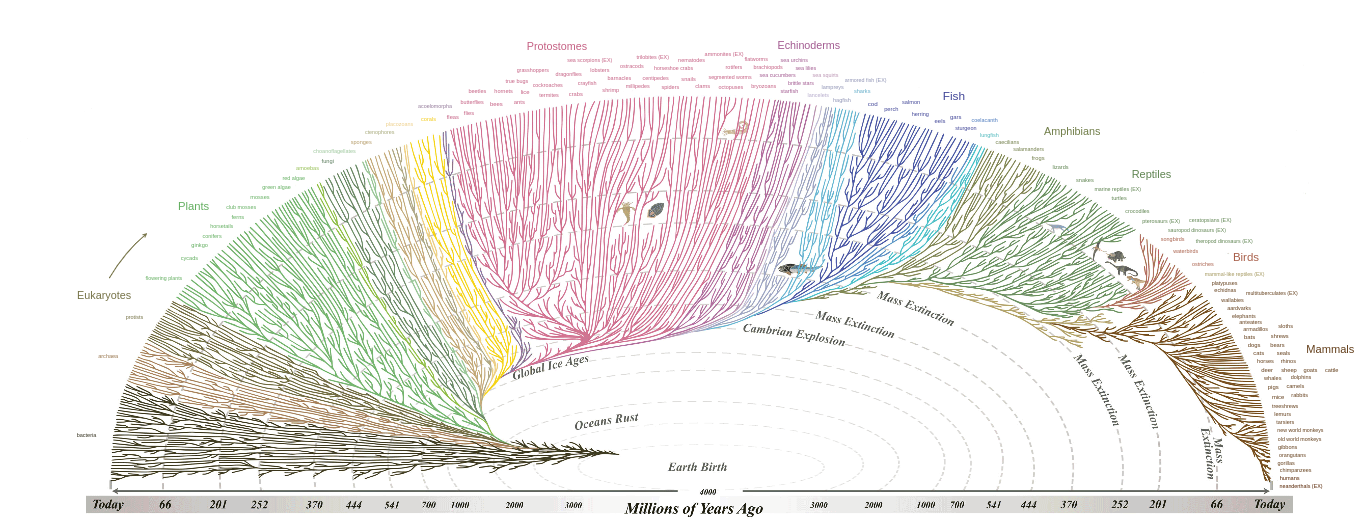
\includegraphics[width=0.45\textwidth]{figures/related_work/evogeneao_overview}\label{fig:evogeneao_a}} 
	\hfill
	\subfigure[The ancestral relationship between human and songbird. ]{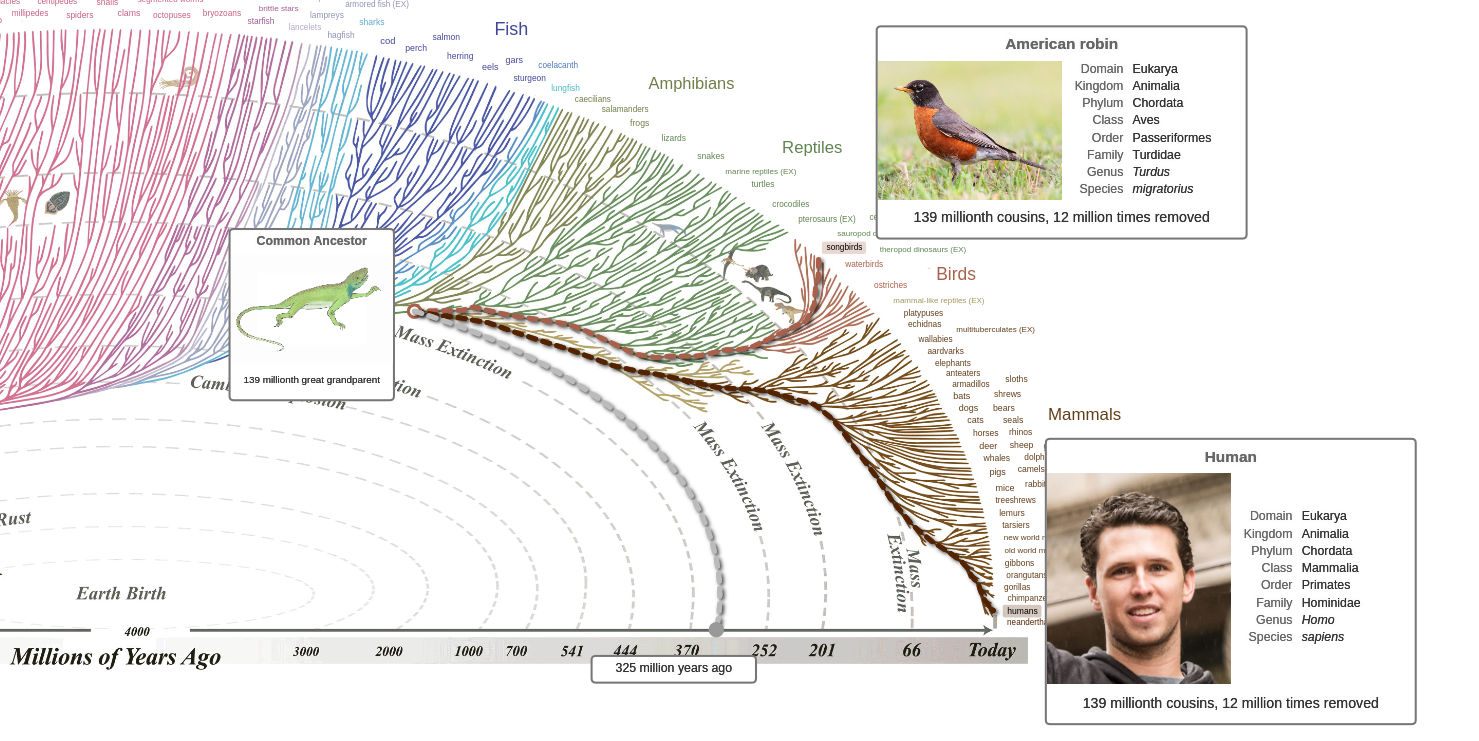
\includegraphics[width=0.45\textwidth]{figures/related_work/evogeneao_relationship}\label{fig:evogeneao_b}} 
	\caption{Tree of life implementation in Evogeneao. }
	\label{fig:evogeneao}
\end{figure}

Finally, there are a wide variety of tree of life visualized for computational biologists. Such visualizations provide rich functionalities for bioinformatic analysis that are well beyond the need of general public and often take efforts to use. An example is iTOL (\url{https://itol.embl.de/itol.cgi},Fig\ref{fig:iTOL}). The design of arranging all leaves on the edge of a circle and all nodes in its interior utilizes space effectively, therefore can be adapted in our implementation. 

\begin{figure}[h]
	\centering
	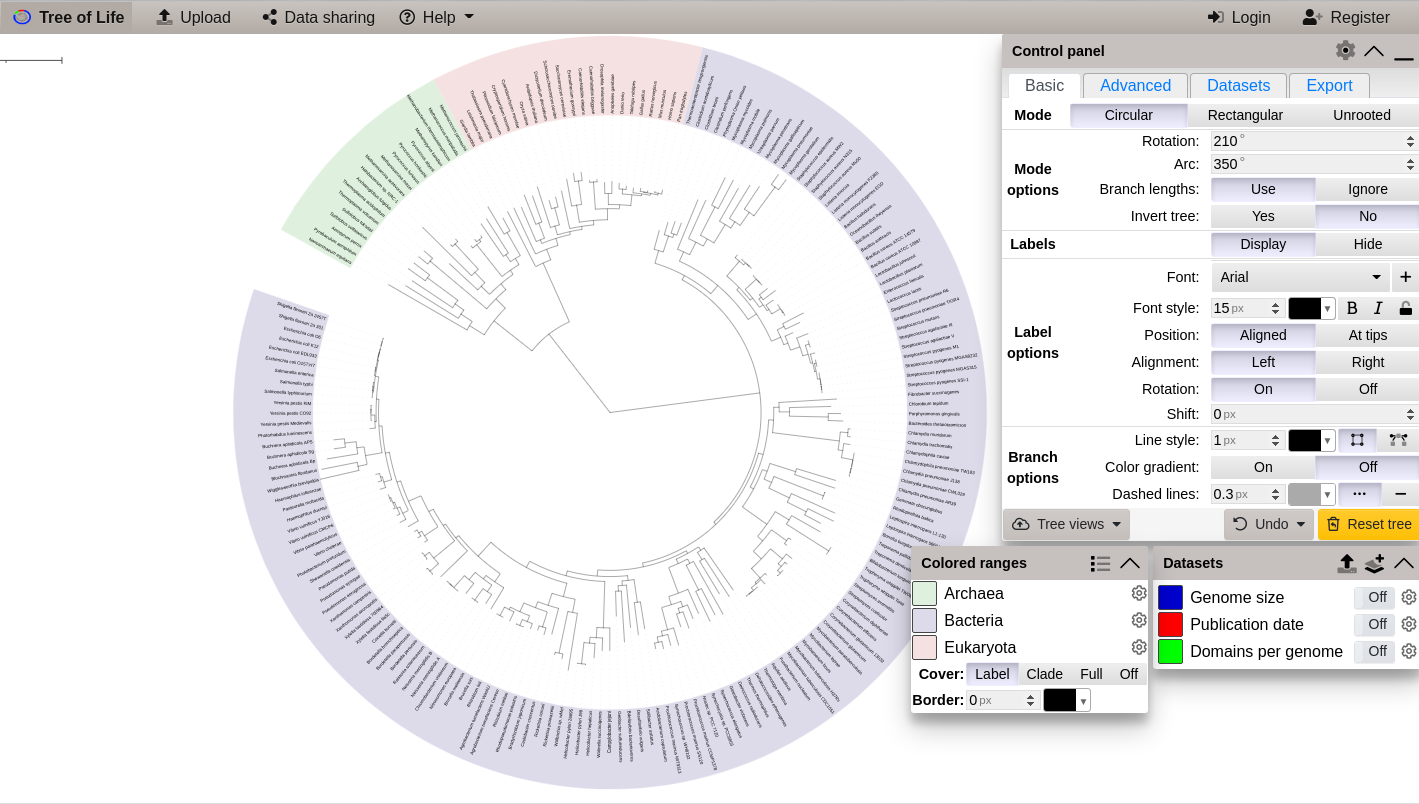
\includegraphics[width=0.5\textwidth]{figures/related_work/iTOL}
	\caption{Tree of life in iTOL. }
	\label{fig:iTOL}
\end{figure}

\section{Visualizations on tectonic shift}
\begin{figure}[h]
	\centering
	\subfigure[Tectonic shift visualized in Ancient Earth. ]{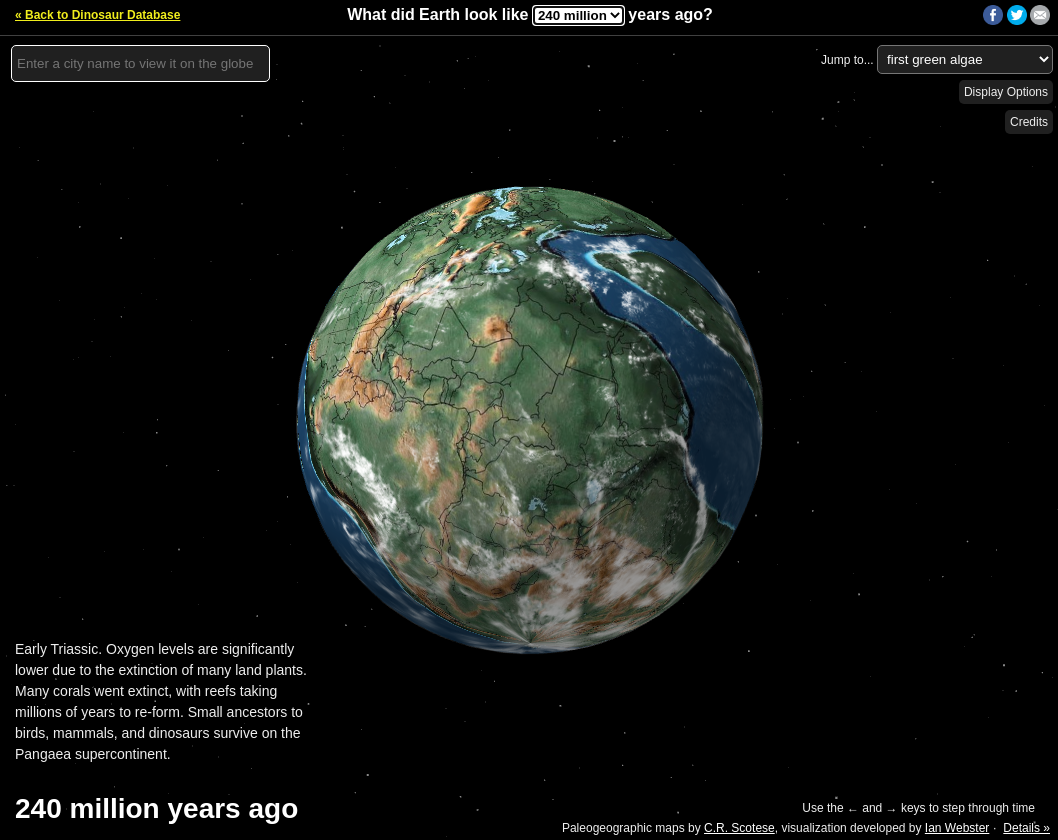
\includegraphics[width=0.45\textwidth]{figures/related_work/ancient_earth}\label{fig:ancient_earth}} 
	\hfill
	\subfigure[Tectonic shift visualized in Earth Viewer. ]{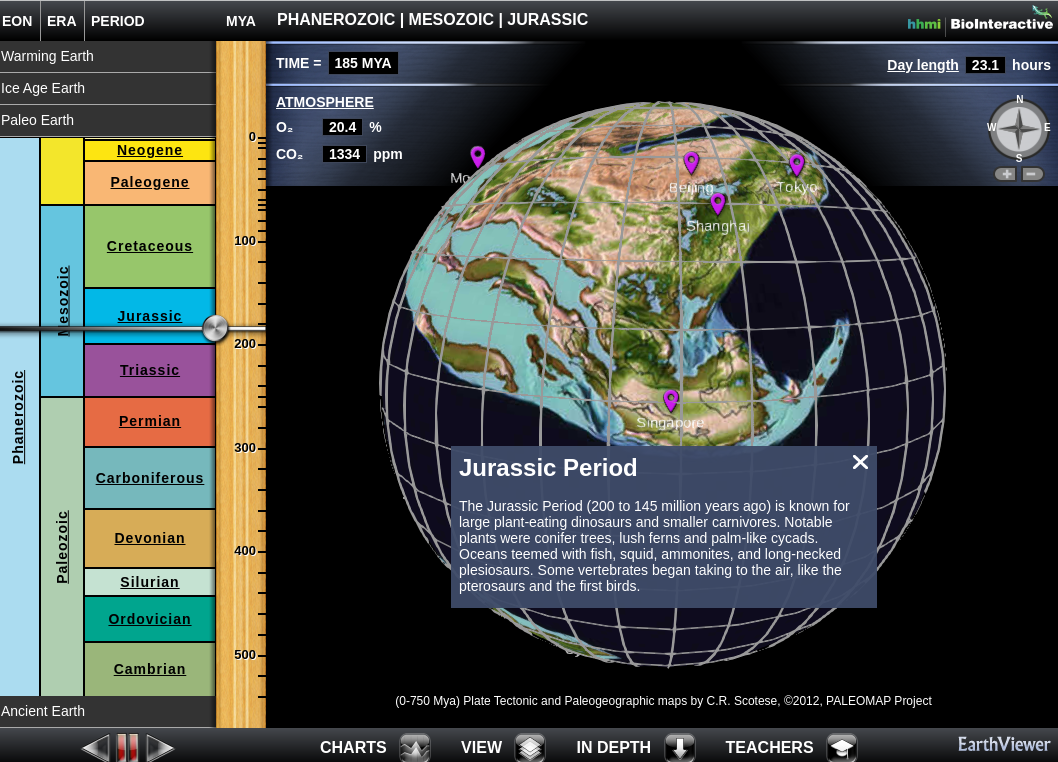
\includegraphics[width=0.45\textwidth]{figures/related_work/earth_viewer}\label{fig:earth_viewer}} 
	\caption{Example visualizations on tectonic shift. }
	\label{fig:tectonic_shift}
\end{figure}
Current project involves visualizing plate motions in various time period, since biodiversity information is shown on the world map during the select time period of interest. Two typical tectonic shift visualizations are Ancient Earth (\url{https://dinosaurpictures.org/ancient-earth#240}, Fig\ref{fig:ancient_earth}) and Earth Viewer (\url{https://www.biointeractive.org/classroom-resources/earthviewer}, Fig\ref{fig:earth_viewer}). Both of them show the coastlines of the continents at a select time point on a three-dimensional globe. Ancient Earth allows users to pick a particular time point from a list of options and search for the ancient location of a city. Earth Viewer provides more detailed information on geological time, and selectable time points are incremented at every five million years on the scroll bar. Time periods are organized in a hierarchical structure with names, which can be adapted in this project for easy navigation. When clicking on a time period, instead of directing the user to the selection, a pop-up window containing a brief introduction of the time period appears, which is counter-intuitive. An improvement is to show the earth at the middle of the selected time period upon clicking.

%=====================================================================
\chapter{Problem statement} \label{chp:problem_statement}
%=====================================================================
The data visualization project is divided into several sub-problems as follows.

\begin{itemize}
	\item \textbf{Data processing}
	\begin{itemize}
		\item Process the PBDB dataset to extract fossil records 
		\item Extract a tree of life from the taxonomy information of the fossil record 
		\item Trace the coordinates of each fossil record to ancient time
	\end{itemize} 
	\item \textbf{Database setup}: store the fossil data, coordinate data and the taxonomy data into a database
	\item \textbf{Back-end building}: enable data queries from the database upon users' request from the front-end 
	\item \textbf{Front-end building}: visualize interactive components for users to explore biodiversity through deep time
	\begin{itemize}
		\item A time component that lists ancient epochs that users can select
		\item A tree component that shows the tree of life constructed by the fossil records found in the selected time period, under the selected taxonomy. 
		\item A map component that shows the shape of the continents in the selected time period, and the locations of the fossil records that constitutes the tree of life in the above component.    
	\end{itemize} 
\end{itemize} 

%=====================================================================
\chapter{Technical solution} \label{chp:technical_solution}
%=====================================================================
\section{Overview}\label{sec:tec_overview}
This section explains the technical solutions to the problems stated in chapter \ref{chp:problem_statement}. To summarize, the project is divided into data processing in section \ref{sec:tec_data_processing}, database setup in section \ref{sec:tec_database_setup}, back-end development in section \ref{sec:tec_backend} and front-end development in section \ref{sec:tec_frontend}, and the workflow of the project follows the same order. 

\begin{figure}[h]
	\centering
	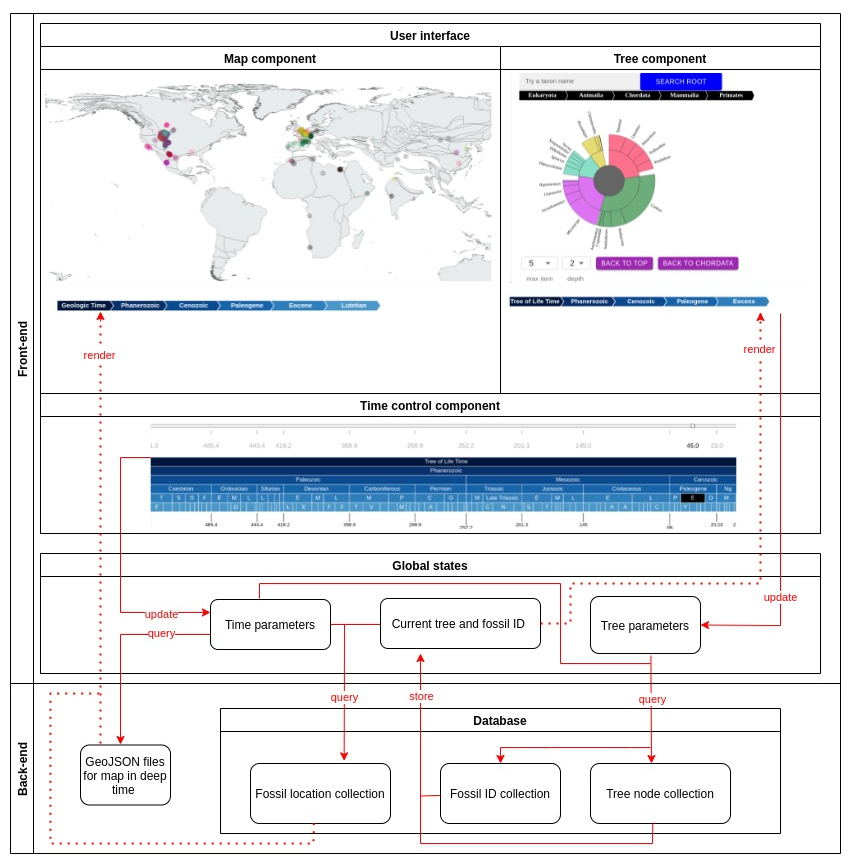
\includegraphics[width=0.9\textwidth]{figures/technical_solution/architecture}
	\caption{An overview of the architecture solution for the project. The user interface consists of a map, a tree and a time table. The global states store tree and time parameters that are customized by users, and the current tree nodes attached with fossil ID sent from database. The back-end resolves queries on tree, fossil locations and map, before sending data back to front-end, where the data is visualized. }
	\label{fig:architecture}
\end{figure}

Diagram \ref{fig:architecture} proposes a structure of the designed visualization system. The front-end of the web application has a user interface and global states section that stores variables accessible to the components of the user interface. The back-end stores data either in database or as static files, and it responds to the data requests by the front-end, by sending data back to global states section for storage, or directly to the user interface for visualization. Map, tree and time control are the three components that users can view and interact with. The time control panel allows users to select a time period to either view the tree of life, or track the fossil location change due to plate motion. The \emph{time parameters} from global states section listen to user-induced changes in the time control panel, and triggers request of map data, tree data (together with tree parameters stored in global states) or fossil location data (together with fossil ID information stored in global states). The map component receives 1, coastline boundary data in GeoJSON format and 2, fossil location data in database at back-end, to render world map and fossils in a selected time period. The tree component shows the tree of life stored in global states. When users customize the tree view, the tree parameters are updated, and new data on tree nodes with attached fossil IDs is queried from the database. The data is returned to the tree and fossil ID storage in global states, which in turn sends only the tree information to the tree component to be rendered as the new tree. 

\section{Data processing} \label{sec:tec_data_processing}
\subsection{Raw data parsing} \label{subsec:raw_data_parsing}
The data source for fossil records and the tree of life is provided by Paleobiology Database (PBDB). The raw data consists of two csv files that contain 1240202 animal fossil records and 105918 plant fossil records, respectively. Since the two files share the same data attributes, the data is concatenated into one file. Only the attributes that are relevant to this project are parsed, which are listed below.\\

\noindent Extracted attributes in the PBDB dataset:
\begin{itemize}
	\item \textit{occurrence\_no}: a unique ID code for a fossil record
	\item \textit{accepted\_name}: the accepted name of a fossil record
	\item \textit{accepted\_rank}: the taxonomic rank in which the accepted\_name belongs to 
	\item \textit{phylum}: the phylum name of the fossil record
	\item \textit{class}: the class name of the fossil record
	\item \textit{order}: the order name of the fossil record
	\item \textit{family}: the family name of the fossil record
	\item \textit{genus}: the genus name of the fossil record
	\item \textit{max\_ma}: the oldest estimated time of the fossil record, in million years
	\item \textit{min\_ma}: the earliest estimated time of the fossil record, in million years
	\item \textit{lng}: the longitude of the fossil record's found location 
	\item \textit{lat}: the latitude of the fossil record's found location 
	
\end{itemize}

In addition, we append a new attribute to the dataset to keep note of which one of the two files a fossil record is originated from: 

\begin{itemize}
	\item \textit{kingdom}: the kingdom name of the fossil record	
\end{itemize}

The kingdom of Animalia and Plantae is assigned to each fossil record, depending on whether it is from the animal or plant file, respectively. \\

By observing the available attributes in the raw data, we can determine how it can be used for an interactive visualization. The biodiversity of a given time period is represented by 1, a dynamic tree of life formed by the fossil records during that time period, and 2, the locations of the fossils on a world map of that time period. The \emph{occurrence\_no} uniquely identifies a fossil record. The \emph{max\_ma} and \emph{min\_ma} together describe during which time period(s) the organism was alive. The \emph{lat} and \emph{lng} are required to calculate the location of a record during an ancient time period. Most importantly, a tree of life is needed to host each fossil record on a specific node. To generate a tree structure, information on parent-child relationship is essential. This relationship is represented in the names on each of the taxonomic ranks, in the descending order of \emph{domain}, \emph{kingdom}, \emph{phylum}, \emph{class}, \emph{order}, \emph{family}, \emph{genus}, \emph{species}. The raw data lacks information on \emph{domain} and \emph{species}. However, since all records are either animals or plants, they all belong to the common domain of Eukaryota. When the value of \emph{accepted\_rank} is species, the species name is found in \emph{accepted\_name}. Therefore, the raw data has sufficient information to construct a tree of life with the eight above-mentioned taxonomic ranks as its levels.\\

The datasets on fossils and tree are created from this parsed raw data. In the next steps, we first prepare the dataset that contains all fossil points, since the tree dataset is created based on it. 

\subsection{Fossil point dataset preparation}
\label{subsec:fossil_preparation}
Since the coordinates of a fossil record depend on the time due to tectonic motion, two datasets are created in regarding to fossil data. This section produces the first dataset \emph{fossil point}, which concerns the taxonomy and the range of age for each record, and sub-section \ref{subsec:geospatial_transformation} produces \emph{fossil location}, the second dataset that stores the coordinates of each fossil record on various time periods in history. \\

The purpose of \emph{fossil point} dataset is to accurately describe a given fossil record in relation to the tree of life, without considering its location at a given time period. The parsed raw data already provides \emph{occurrence\_no}, a unique ID code, as well as \emph{max\_ma} and \emph{max\_ma}, which indicate its range of age in million years. However, one more attribute is required to describe its taxonomy, such that it can be attached to a particular node in the tree of life to be constructed in the next step. This attribute is essentially the unique identifier of a node in the tree of life, and will also serve as the link between the fossil point dataset and the tree dataset. Although it is natural to consider \emph{accepted\_name} and \emph{accepted\_rank} in the parsed raw data for this purpose, they cannot be used for the following reasons. Firstly, \emph{accepted\_name} and \emph{accepted\_rank} does not correlate well with the names on the taxonomic ranks, as some \emph{accepted\_rank} does not belong to any of the eight ranks that will be used in the tree of life. As a consequence, some fossil records cannot be assigned to the tree, since the \emph{accepted\_name} values corresponding to the \emph{accepted\_rank} will not be found in the tree. Secondly, the \emph{accepted\_rank} and \emph{accepted\_name} attributes are not unique. For instance, the genus "Banksia" is both an animal taxonomy and a plant taxonomy. In such cases, fossil records can be associated to a incorrect branch if only these two pieces of information is used. Thirdly, many names in the taxonomic ranks are missing. This leads to ambiguity when attaching a particular fossil to the tree of life, when there exists a rank above the \emph{accepted\_rank} with missing names. An example is shown below.

\begin{table}[h]
	\centering
	\begin{tabular}{|l|l|l|l|l|l|l|l|l|l|}
		\hline
		occurrence\_no &  accepted\_name & accepted\_rank & kingdom &	phylum & class & order & family & genus & ... \\ \hline
		3285 &  Tetradium & genus & Plantae & Rhodophyta & NaN & NaN & NaN & Tetradium & ... \\ \hline
	\end{tabular}
	\caption{An example row of parsed raw data with missing information.}
	\label{tab:missing_information}
\end{table}

With only the \emph{accepted\_name} "Tetradium" on the \emph{accepted\_rank} "genus", we are uncertain about which class, order or family to associate this fossil record to under the phylum of "Rhodophyta". Extra knowledge in taxonomy is needed to retrieve the missing names on the path from "Rhodophyta" to "Tetradium" and this challenge is beyond the scope of the current project. The current solution only attaches the fossil record "3285" to the phylum of "Rhodophyta" and ignores its taxonomy below the phylum level. \\

To solve these three issues and provide a method for uniquely identifying a fossil record to the tree without ambiguity, the attributes \emph{path\_from\_root} and \emph{rank} are introduced. 

\begin{itemize}
	\item \textit{path\_from\_root}: a comma separated string indicating the path from the root Eukaryota to the name on lowest possible taxonomic rank with no missing names in between
	\item \textit{rank}: the lowest taxonomic rank of \textit{path\_from\_root}
\end{itemize}

Since a path begins from the common root Eukaryota and terminates when reaching the lowest rank level "species", or encountering a missing name, the example in Table \ref{tab:missing_information} has "Eukaryota, Plantae, Rhodophyta" as \emph{path\_from\_root} and "phylum" as \emph{rank}. All names in \emph{path\_from\_root} are guaranteed to be present in the tree, since the names are taken from the same taxonomy information that is used to construct the tree. The path from the common root Eukaryota describes the exact location of a node in the tree, which serves as the node's unique identifier. In addition, the fossils associated to the subtree under a certain taxonomy can be easily obtained by string matching this path using regular expression. \\

To calculate \emph{path\_from\_root} and \emph{rank}, the following attributes are used:  \emph{domain}, \emph{kingdom}, \emph{phylum}, \emph{class}, \emph{order}, \emph{family}, \emph{genus}, \emph{accepted\_name}, \emph{accepted\_rank}. Instead of iterating over each row in the parsed raw data, we first aggregate the rows when those values are identical and then perform the iteration, before joining the result with the original data (similar to an "inner join" operation in SQL), in order to avoid repetitive computation. \\

At each iteration process on the aggregated data, we initialize the \emph{path\_from\_root} as "Eukaryota" and visit each taxonomic rank from \emph{kingdom} to \emph{genus}, while appending a comma and the name on each rank to the end of the string and updating the current rank. The iteration terminates at the first missing name, when both \emph{path\_from\_root} and \emph{rank} are those of the missing name's parent. After visiting \emph{genus}, the iteration finishes when the \emph{accepted\_rank} is "genus". Otherwise, the \emph{accepted\_rank} is "species" or "subspecies". Under this circumstance, we append the value of \emph{accepted\_name} to \emph{path\_from\_root}, update \emph{rank} to be the value of \emph{accepted\_rank}, and terminate the iteration. The name in the path after genus can thus be either a species or a subspecies, which is acceptable, since a subspecies name already includes the species name (\emph{i.e.}, the species name of the subspecies "Argopecten circularis impostor" is "Argopecten circularis"). \\

It is important to note that the columns \emph{path\_from\_root} and \emph{rank} are precursors to the tree dataset, since they represent all nodes with at least one fossil record attached. The unique values of the two columns are used for further processing in sub-section \ref{subsec:tree_preparation}. In the meantime, the aggregated data with \emph{path\_from\_root} appended are joined with parsed raw data, such that every fossil record has a path. Finally, the \emph{fossil point} dataset is generated, by extracting the following attributes: 

\begin{itemize}
	\item \textit{occurrence\_no}
	\item \textit{path\_from\_root}
	\item \textit{max\_ma}
	\item \textit{min\_ma}
\end{itemize}


\subsection{Tree dataset preparation} \label{subsec:tree_preparation}
The purpose of the \emph{tree} dataset is to describe every node on the tree of life that can also be easily searched. The following attributes are computed: \\

\begin{itemize}
	\item \textit{path\_from\_root}: a comma separated string indicating the path from the root Eukaryota to the name on lowest possible taxonomic rank with no missing names in between
	\item \textit{parent}: the \textit{path\_from\_root} of its parent
	\item \textit{name}: the name of the node
	\item \textit{is\_leaf}: a boolean value that indicates if the node is a leaf node
	\item \textit{max\_ma}: the earliest age in million years of the fossils in the subtree of this node
	\item \textit{min\_ma}: the latest age in million years of the fossils in the subtree of this node
\end{itemize}

For each node, we need a unique identifier, which is provided by \emph{path\_from\_root} as discussed in the above sub-section \ref{subsec:fossil_preparation}. The last \emph{name} of the path is also extracted as an attribute, enabling a more convenient node search when users type a name in the search bar. The node's parent attribute allows searching for all children of a given node. The \emph{is\_leaf} attribute indicates directly whether or not a node has children without searching for them. Lastly, \emph{max\_ma} and \emph{min\_ma} provide a quick way to tell if a node is present during a given time period without searching for fossils attached to its subtree. \\

To prepare this dataset, we start from the precursor dataset from \ref{subsec:fossil_preparation}, which has two columns: \emph{path\_from\_root} and \emph{rank}. As a reminder, the \emph{path\_from\_root} are the unique identifiers of all nodes in the tree with at least one fossil record attached. However, there are more nodes to include in the tree. For each entry in the tree represented by its \emph{path\_from\_root}, we must also include each of the upstream ancestor in the tree. For instance, when the node "a,b,c,d" exists, its ancestors "a,b,c", "a,b" and "a" should also be included in the tree. Therefore, the first step is to add the missing nodes. We iterate every \emph{path\_from\_root} to add all ancestors along each path to the data. Given a path, the \emph{path\_from\_root} values of all its ancestors are simply strings sliced from the beginning of the path, until each of its commas. The \emph{rank} value of an ancestor can also be computed by counting the number of commas in the path, as a "domain" has no comma in its path, and a "genus" has six commas. After the iteration, only the unique \emph{path\_from\_root} and the corresponding \emph{rank} values are kept to avoid duplicates.\\

The \emph{parent} and \emph{name} values can be easily extracted from a \emph{path\_from\_root}. The common root "Eukaryota" has no parent, and any other node's parent is represented by the substring of its \emph{path\_from\_root} sliced until the last comma. Similarly, the \emph{name} of a node is the sub-string beginning from the first character after the last comma in its path. Next, we visit each \emph{path\_from\_root} once again. If the path is in the set of all \emph{parent} values, then this node is not a leaf node, and its \emph{is\_leaf} value is set to be "False", otherwise "True". \\

Finally, we calculate the \emph{max\_ma} and \emph{min\_ma} values for each node, using the processed fossil data from \ref{subsec:fossil_preparation}, which now contains the path name and the age range information for each fossil record. We first create a reference dataset, by grouping the fossil data by the same \emph{path\_from\_root} on two attributes: 1, maximum of \emph{max\_ma} values among the fossils with identical path and 2, minimum of \emph{min\_ma} values. Next, we iterate through this reference dataset. For each path, we extract all its ancestors using the same string splitting method as mentioned above, visit those ancestors in the tree dataset, and 1, update its \emph{max\_ma} only if it is less than the current \emph{max\_ma} of the path under iteration and 2, update its \emph{min\_ma} only if it is greater than the current \emph{min\_ma} of the path under iteration.

\subsection{Geospatial transformation of map and fossil data} \label{subsec:geospatial_transformation}
Apart from the tree, a major component of the visualization is a world map responsive to time selection, on which the locations of the fossils are also shown. Therefore, given a geological timescale, we need to calculate the world maps in all time periods. For each fossil point, its coordinates during those time periods are also calculated and stored in the \emph{fossil\_location} dataset. \\

The timescale data is provided by PBDB. Similar to the tree of life, it is also hierarchical, with five layers in total. The highest layer Phanerozoic ranges from 541 million years ago to present time, and the intervals on the fifth layer often spans only several million years. Nevertheless, plates move constantly, such that the location of a given point at the end of a time interval varies from the location at the start of the interval, even if this interval is in the fifth layer of the timescale.  Our solution is to represent the geology of a time period using the middle value of a certain fifth-layer interval. When the user select a time interval in the fifth layer, the coordinates are transformed to that of the interval's middle time point rounded to an integer. When a higher-layer time interval is selected, we first find the fifth-layer in which the middle value of the selected interval falls into, before transforming the coordinates to the integer time point in the middle of that fifth-layer interval. \\

Both the global plate boundaries of modern day and the model to transform a modern location to an ancient one are provided by Matthew \emph{et al.} \cite{matthews2016global}. In this paper, they proposed a high-resolution model on the movement of plates from late Paleozoic (410 million years ago) to modern day. The boundaries of plates that form the coastlines of a world map, as well as the fossil points belonging to their respective plates, can thus be transformed to a desired time point no earlier than 410 million years ago. In the parsed raw PBDB data from sub-section \ref{subsec:raw_data_parsing}, we extract the \emph{lat} and \emph{lng} attributes as the modern coordinate of a fossil point, and \emph{occurrence\_no} as the ID for each fossil point. For each time point, the model transforms both the modern plate boundaries and the modern locations of each fossil record to their ancient coordinates. Finally, the map data is stored as GeoJSON files, and the ancient locations of each fossil point is stored in the \emph{fossil\_location} dataset with the following attributes: \\

\begin{itemize}
	\item \textit{occurrence\_no}: the ID of a fossil record
	\item \textit{mya}: the time point as an integer in million years
	\item \textit{lat}: the latitude of the fossil record in the corresponding time point
	\item \textit{lng}: the longitude of the fossil record in the corresponding time point
\end{itemize}

\section{Database setup} \label{sec:tec_database_setup}
The fossil and tree information are stored in a database, from which requested data is sent for visualization according to queries generated from user interactions. The three prepared datasets are uploaded to the database, with slight renaming and reorganizing in the following manner:

\begin{itemize}
	\item \textit{fossilLocation}: It stores the \textit{fossil location} dataset, which contains the locations at different time points for each fossil record. It has the following fields: \textit{id} (\textit{occurrence\_no} from \textit{fossil location}), \textit{mya} (\textit{mya} from \textit{fossil location}), \textit{coordinates} (an array of [\textit{lat},\textit{lng}] from \textit{fossil location}).
	\item \textit{fossilPoint}: It stores the \textit{fossil point} dataset, which contains taxonomy and range of age for each fossil record. It has the following fields: \textit{id} (\textit{occurrence\_no} from \textit{fossil point}), \textit{maxma} (\textit{max\_ma} from \textit{fossil point}), \textit{minma} (\textit{min\_ma} from \textit{fossil point}), \textit{pathFromRoot} (\textit{path\_from\_root} from \textit{fossil point}).
	\item \textit{TreeNode}: It stores the \textit{tree} dataset, which contains each node in the tree of life. It has the following fields: \textit{pathFromRoot} (\textit{path\_from\_root} from \textit{tree}), \textit{maxma} (\textit{max\_ma} from \textit{tree}), \textit{minma} (\textit{min\_ma} from \textit{tree}), \textit{parent} (\textit{parent} from \textit{tree}), \textit{name} (\textit{name} from \textit{tree}), \textit{isLeaf} (\textit{is\_leaf} from \textit{tree}).
\end{itemize}

An entity relationship is shown in Figure \ref{fig:er}. \emph{FossilLocation} is linked to \emph{FossilPoint} via \emph{id}, the unique identifier for a fossil record. An instance of \emph{FossilPoint} can relate to many instances of \emph{FossilLocation}, because a fossil point has many locations in various time points. An instance of \emph{FossilLocation} relates to one and only one fossil record in \emph{FossilPoint}. An instance of \emph{FossilPoint} is uniquely identified by its \emph{id}. \emph{FossilPoint} and \emph{TreeNode} are linked via \emph{pathFromRoot}. One fossil record is associated to one and only one node in \emph{TreeNode}, however, a tree node can have zero or many fossil records. Indeed, a tree node of a high taxonomic rank has no fossil attached to it, when all fossils under this taxonomy are identified with a lower rank, thus are attached to its descendants. For instance, the root node "Eukaryota" has no fossil attachment, since for any given fossil, we have at least identified it as an animal or a plant. Finally, an instance of \emph{TreeNode} represents a certain node in tree of life, therefore is uniquely identified by its \emph{pathFromRoot}.
\begin{figure}[h]
	\centering
	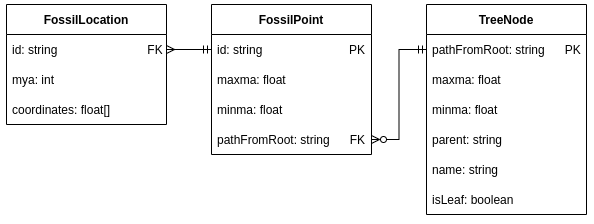
\includegraphics[width=0.4\textwidth]{figures/technical_solution/er}
	\caption{An entity relationship diagram of the database.}
	\label{fig:er}
\end{figure}

\section{Back-end query processing} \label{sec:tec_backend}
The back-end is responsible for processing the data queries requested by user actions, and sending the result to the front-end. How the queries are resolved is addressed in this sub-section. There are two main queries to carry out: 1, given a time range and tree parameters, obtain a tree of life with fossil IDs attached to each node, and 2, obtain the locations of the fossil records given their IDs and a time point. \\

The first query returns a fossil-attached tree under a requested root node. The following parameters are passed to the database: 
\begin{itemize}
	\item \textit{pathFromRoot}: the unique identifier of the root node
	\item \textit{name}: the root node's name
	\item \textit{maxma}: the start of the selected time period
	\item \textit{minma}: the end of the selected time period
	\item \textit{maxElement}: the maximum number of siblings to retrieve
	\item \textit{depth}: the number of tree layers to retrieve 
\end{itemize}

The resulted tree should be rooted by the requested node, with a depth no greater than the parameter \emph{depth}. The number of children under each node is no greater than number of \emph{maxElement}. The IDs of fossils that exist during the time period is also attached to each node. The returned tree has the following attributes:  

\begin{itemize}
	\item \textit{pathFromRoot}: the unique identifier of the node
	\item \textit{name}: the node's name
	\item \textit{parent}: the \textit{pathFromRoot} value of its parent
	\item \textit{isLeaf}: a boolean value indicating if the node is a leaf node in the returned tree
	\item \textit{fossils}: the IDs of fossil records existing during the requested time period that either are attached to this node (if the node is not a lead node) or belong to the node's subtree (if the node is a lead node)
\end{itemize}

To retrieve the tree, we first find the requested root node by searching for its name in \emph{TreeNode}. The \emph{parent} value of the root node is set to null, since although it may have a parent in the complete tree of life, it is the root with respect to the tree to be returned. The fossil IDs attached to the root node is also appended. We then recursively search for its children and append the nodes to the result, until reaching the requested depth, or encountering nodes with no children left. When processing the children of a certain node during the recursion, we check the \emph{isLeaf} value in the following way. If this node has no children, then it is certain a leaf. However, if the node is on the maximum depth, then it is a leaf node with respect to the tree under construction, whether or not it has children in the complete tree of life. When it is a leaf node, we search for the IDs of all fossils belonging to its subtree. This can be easily performed with string matching the \emph{pathFromRoot} of the fossil records using regular expression, since all desired fossils' paths beigin with the \emph{pathFromRoot} of the current node. When the node is not a leaf node, we only attach fossils that are strictly associated with this node, by exact string matching of \emph{pathFromRoot} between this node and the fossil records. To improve efficiency, the sibling nodes are filtered before continuing to the next recursion level. A count value is assigned to each sibling node, which is the number of fossil records in \emph{FossilPoint} belonging to its subtree that is present during the time period. Then the siblings are ranked in descending order, and the top \emph{maxElement} number of siblings are kept. \\

The second query receives a time point of interest and an array of nodes in the current tree, which is a result of the first query. However, only the relevant fields are passed: 
\begin{itemize}
	\item \textit{name}: the node's name
	\item \textit{fossils}: the IDs of fossils attached to the node (if it is a lead node) or its subtree (if it is not a leaf node)
\end{itemize}

From \emph{FossilLocation}, we retrieve the fossils' coordinates by their IDs and time point, and organize the result in the following manner:

\begin{itemize}
	\item \textit{id}: the fossil record's ID
	\item \textit{coordinate}: the fossil location at the time point, in the form of [latitude, longitude]
	\item \textit{name}: the name to which the fossil record is associated in the current tree
	\item \textit{mya}: the requested time point 
\end{itemize}

\section{Front-end development} \label{sec:tec_frontend}
\subsection{The global states}\label{subsec:tec_frontend_global_states}
\subsection{The user interface: time control component}\label{subsec:tec_frontend_time}
\subsection{The user interface: tree component}\label{subsec:tec_frontend_tree}
\subsection{The user interface: map component}\label{subsec:tec_frontend_map}


%=====================================================================
\chapter{Implementation} \label{chp:implementation}
%=====================================================================
\section{Code structure} \label{sec:implementation_code_structure}
\section{Data processing stacks}\label{sec:implementation_data_processing}
\section{Web development stacks}\label{sec:implementation_web_development}

%=====================================================================
\chapter{Results} \label{chp:results}
%=====================================================================
\section{Data analysis} \label{sec:result_data_analysis}
\subsection{fossil data} \label{subsec:data_analysis_fossil}
\subsection{tree data} \label{subsec:data_analysis_tree}

\section{Data visualization} \label{sec:result_data_visualization}
\subsection{Time selector component} \label{subsec:data_visualization_time}
\subsection{Map component} \label{subsec:data_visualization_map}
\subsection{Tree component} \label{subsec:data_visualization_component}
%=====================================================================
\chapter{Conclusion} \label{chp:discussion_conclusion}
%=====================================================================



\section{Limitations and Future Work}

%=====================================================================
\chapter*{Acknowledgements}
%=====================================================================


\bibliographystyle{alpha}
\bibliography{references}

\listoffigures
\listoftables
%=====================================================================
\end{document}

